\documentclass{extarticle}
\usepackage[letterpaper, portrait, margin=1in]{geometry} 
\usepackage{tikz}
\usepackage{tikz-qtree}
\usetikzlibrary{shapes}
\usepackage{graphicx}
\usepackage{amsmath}
\usepackage{amsfonts}
\usepackage{amssymb}
\usepackage{amsthm} % theorem package
\usepackage[utf8]{inputenc}
\usepackage{amsthm}
\usepackage{algorithm}
\usepackage[noend]{algpseudocode}
\usepackage[english]{babel}
\theoremstyle{definition}
\newtheorem{theorem}{Theorem}[section]
\theoremstyle{definition}
\newtheorem{definition}{Definition}[section] % define definition

%%% package used by Xiaoli
\usepackage{verbatim}
\usepackage{hyperref}
\usepackage{subfigure}
\usepackage{listings} %% for display code
\usepackage{hyperref} %% add hyperlink
\usepackage{graphicx}
\usepackage{float}




\begin{document}
\title{Homework 2: Texture Synthesis and Image Inpainting \\
	Computer Vision}
\author{Xiaoli He}
\maketitle
\newpage

%%%%%%%%%%%%%%%%%%%%%%%%%%%%%%%%%%%%%%%%%%%%%%%%%%%%%%%%%%%%%%%%%
\section{Texture Synthesis}
The synthesized images for T1,T2,..., T5.gif by with WindowSize = 5, 9 ,11, 15,23 pixels are shown in Figure \ref{fig_syth}. The average run time was about 6 min. (To filled a 200*200 pixel image).

I also tried window size of 15 and 23 pixels, and the effects are different for different examples. For example, 15 pixels worked best for T1, 23 pixels worked best for T5, and for the rest, increasing window size didn't help significantly. In general, if the texture is more complicated, increasing window size helps. 

Note: the size of each synthesized images are the same (200 *200 pixels), the appeared sizes are different in Figure \ref{fig_syth} due to Latex typesetting...
\begin{figure}[H]
	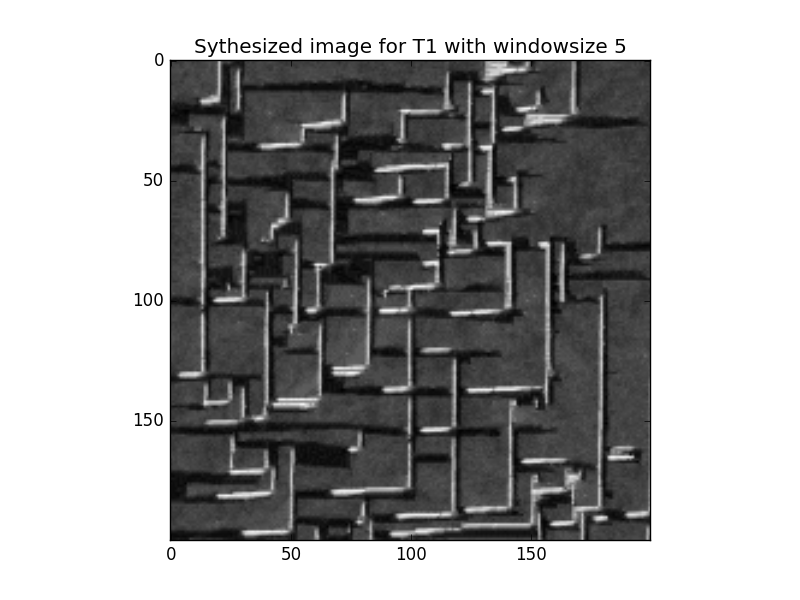
\includegraphics[width = 0.19\textwidth]{./figures/Syth_T1_size_5.png}
	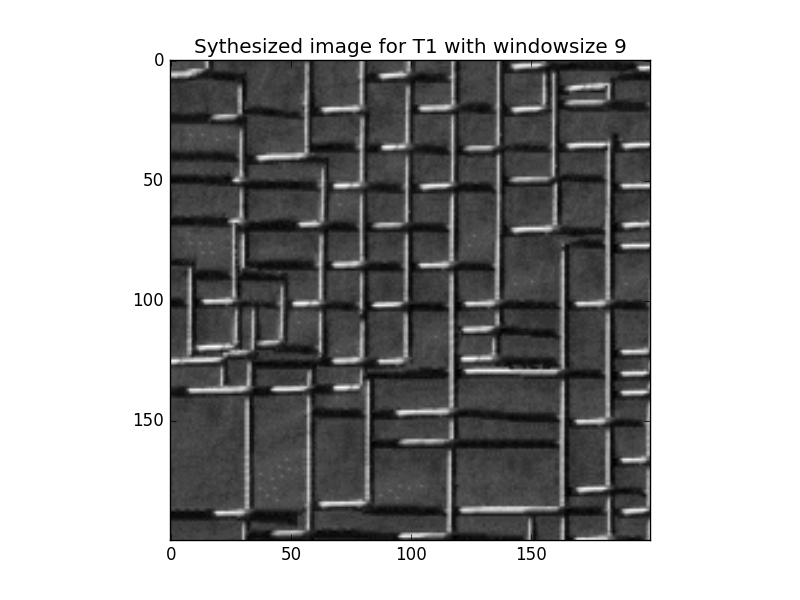
\includegraphics[width = 0.19\textwidth]{./figures/Syth_T1_size_9.png}
	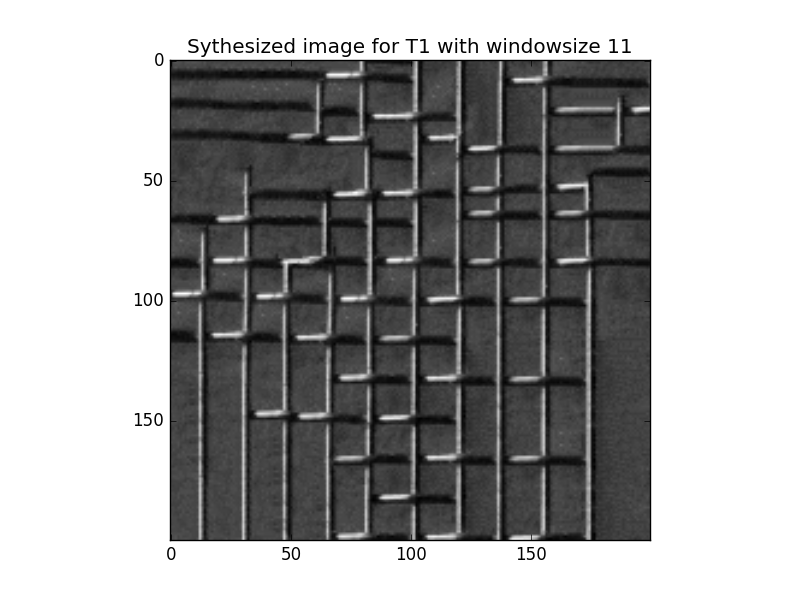
\includegraphics[width = 0.19\textwidth]{./figures/Syth_T1_size_11.png}
	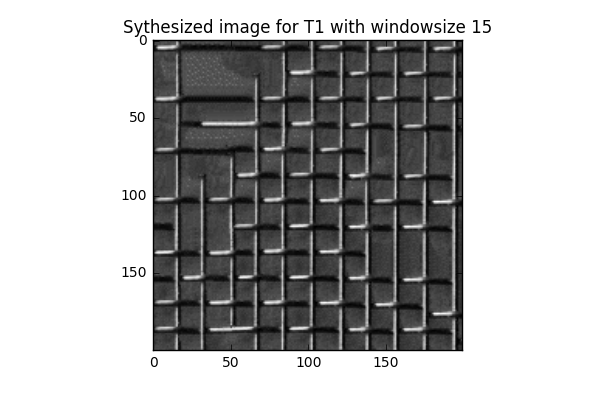
\includegraphics[width = 0.19\textwidth]{./figures/Syth_T1_size_15.png}	
	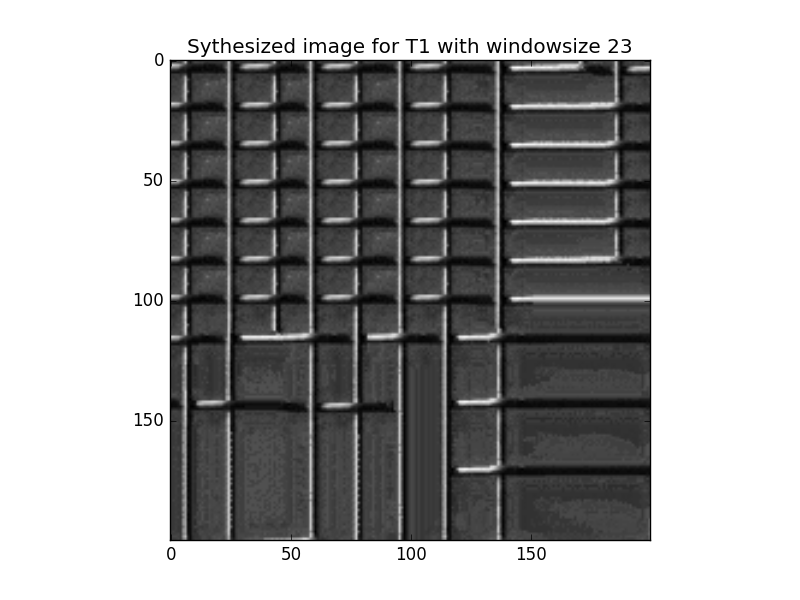
\includegraphics[width = 0.19\textwidth]{./figures/Syth_T1_size_23.png}
	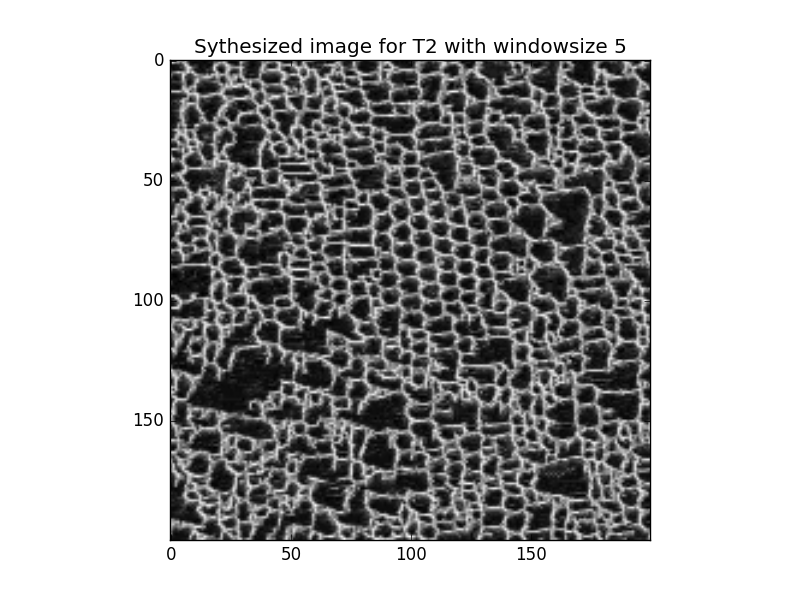
\includegraphics[width = 0.19\textwidth]{./figures/Syth_T2_size_5.png}
	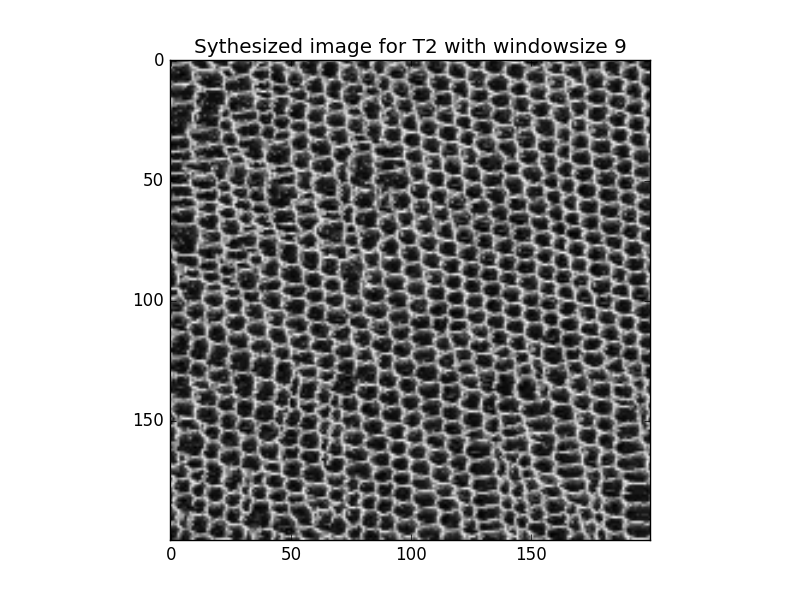
\includegraphics[width = 0.19\textwidth]{./figures/Syth_T2_size_9.png}
	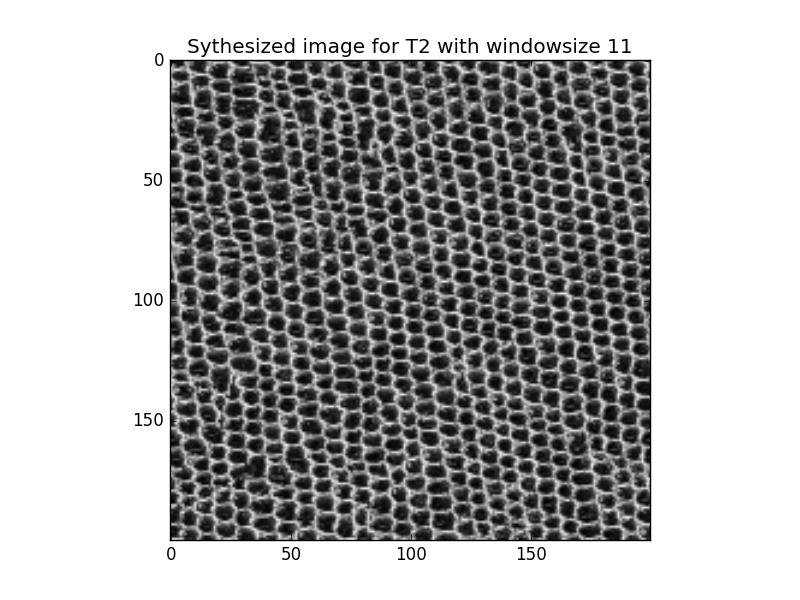
\includegraphics[width = 0.19\textwidth]{./figures/Syth_T2_size_11.png}
	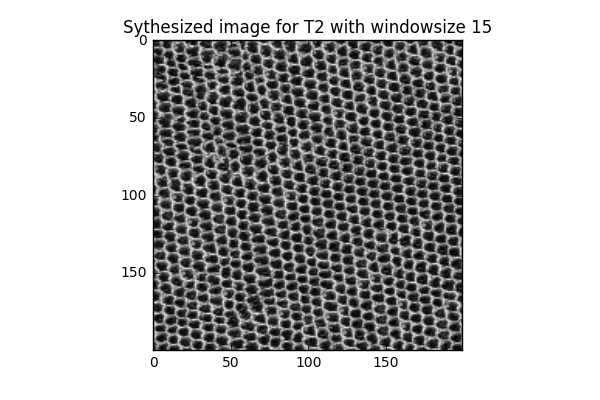
\includegraphics[width = 0.19\textwidth]{./figures/Syth_T2_size_15.png}
	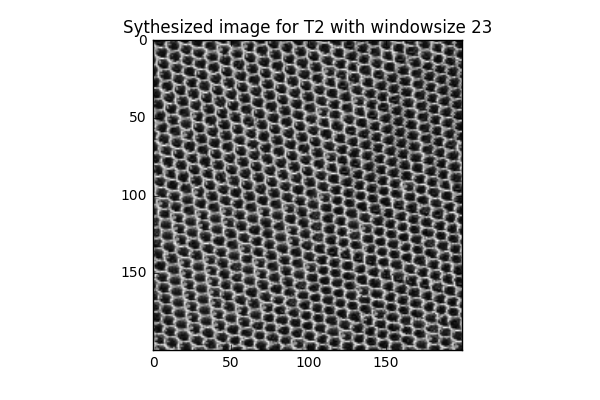
\includegraphics[width = 0.19\textwidth]{./figures/Syth_T2_size_23.png}
	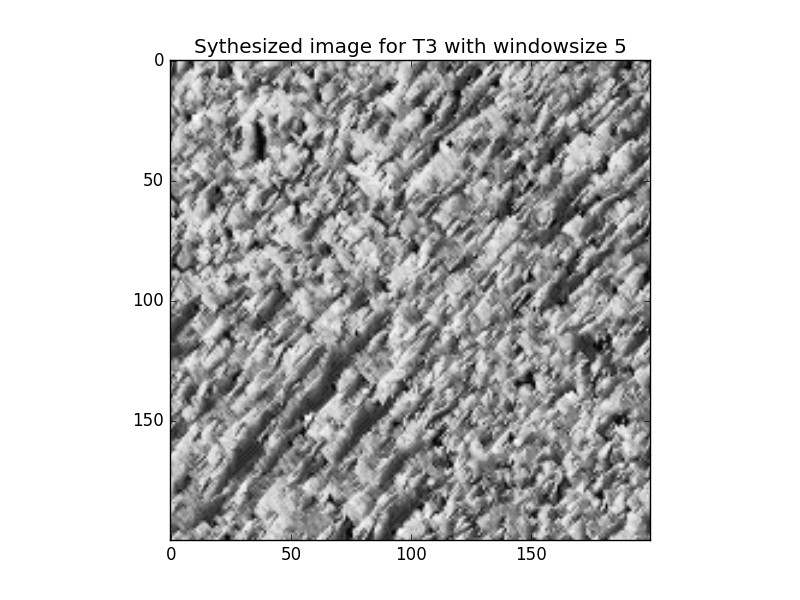
\includegraphics[width = 0.19\textwidth]{./figures/Syth_T3_size_5.png}
	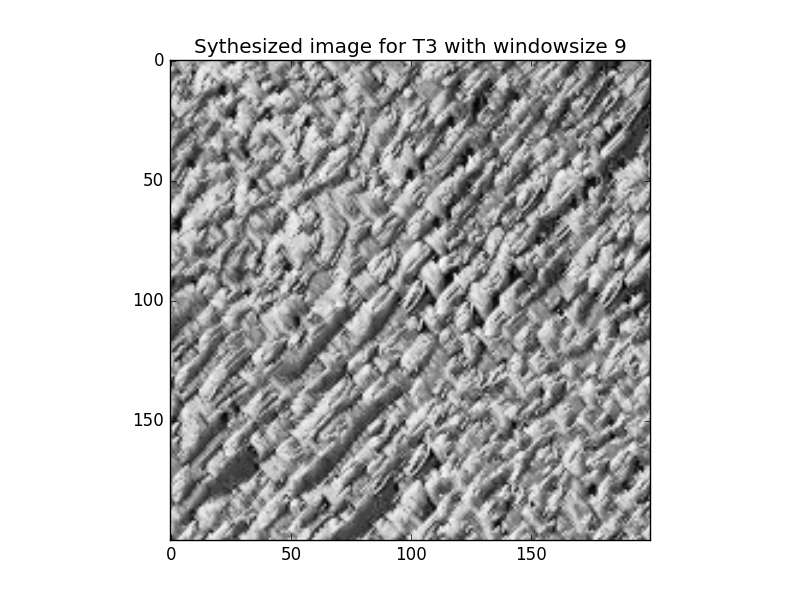
\includegraphics[width = 0.19\textwidth]{./figures/Syth_T3_size_9.png}
	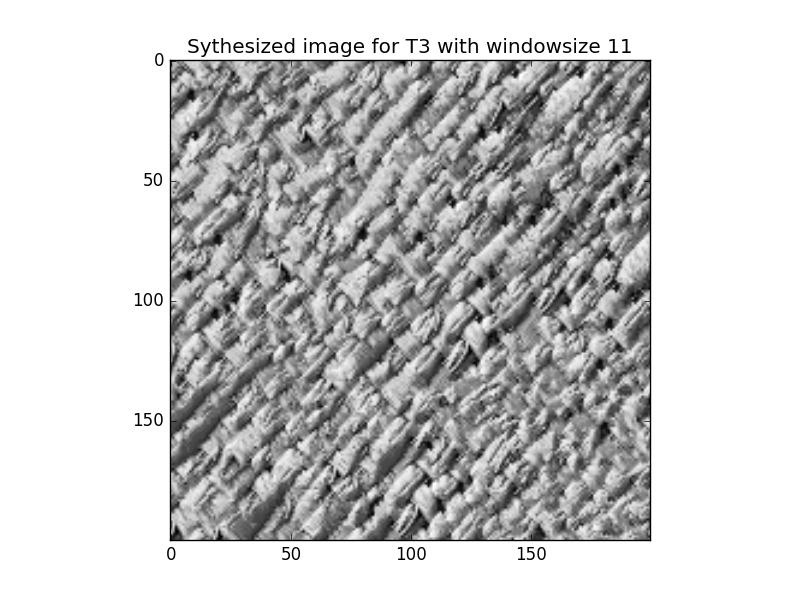
\includegraphics[width = 0.19\textwidth]{./figures/Syth_T3_size_11.png}	
	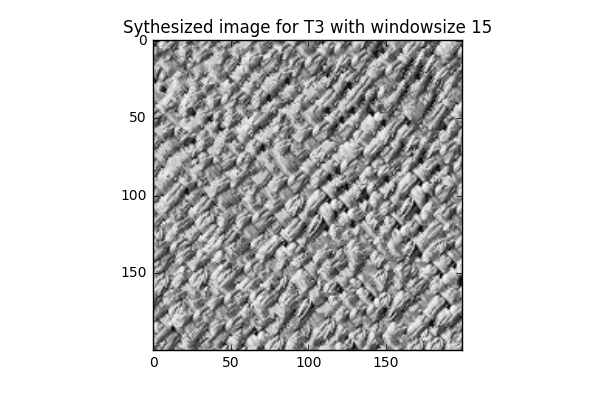
\includegraphics[width = 0.19\textwidth]{./figures/Syth_T3_size_15.png}	
	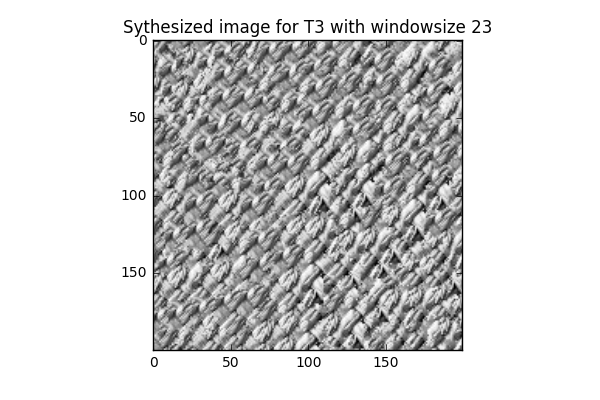
\includegraphics[width = 0.19\textwidth]{./figures/Syth_T3_size_23.png}
	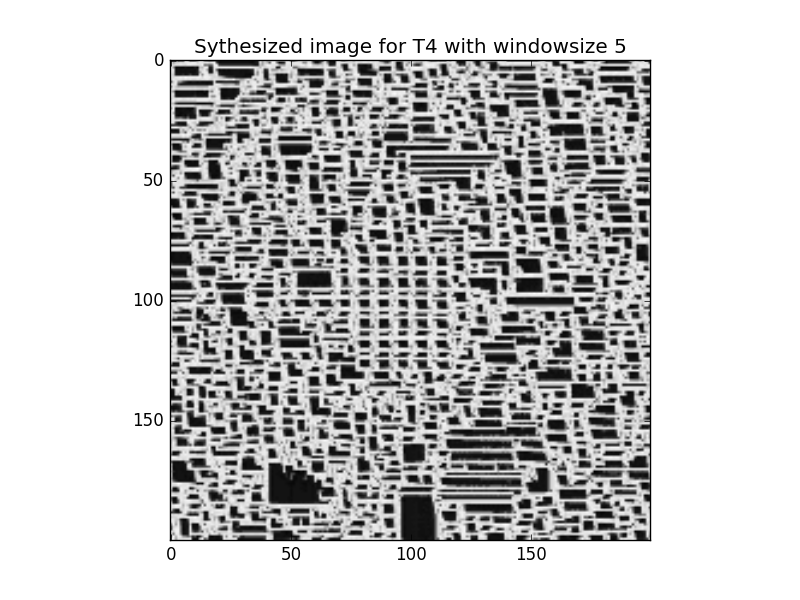
\includegraphics[width = 0.19\textwidth]{./figures/Syth_T4_size_5.png}
	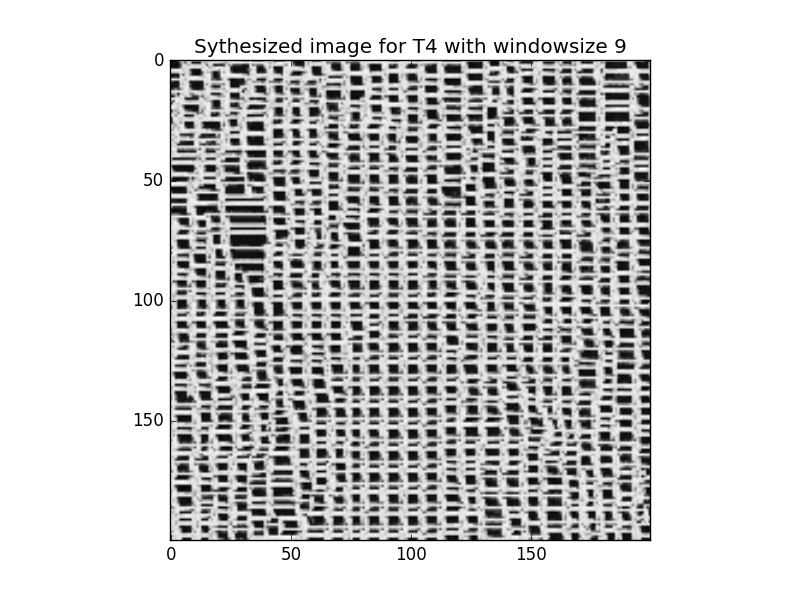
\includegraphics[width = 0.19\textwidth]{./figures/Syth_T4_size_9.png}
	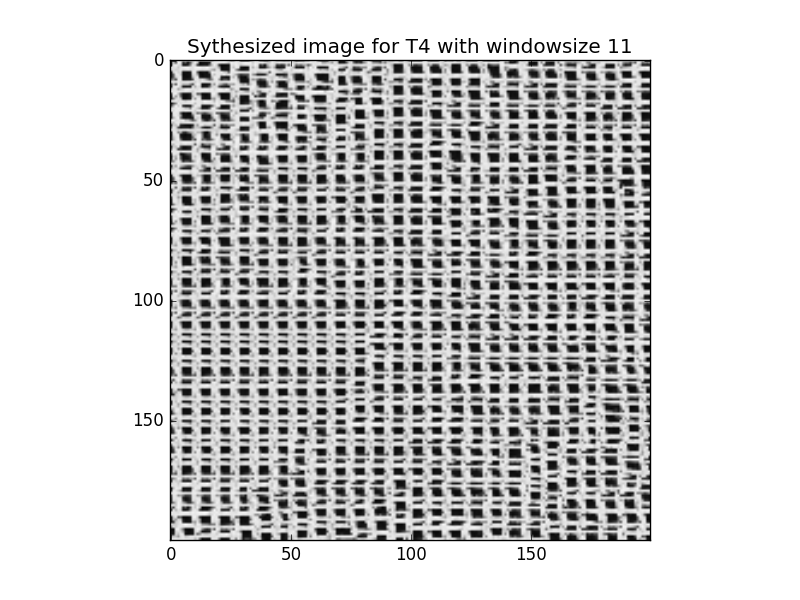
\includegraphics[width = 0.19\textwidth]{./figures/Syth_T4_size_11.png}	
	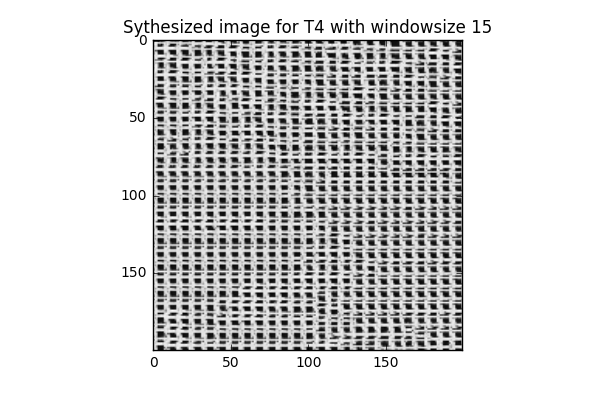
\includegraphics[width = 0.19\textwidth]{./figures/Syth_T4_size_15.png}	
	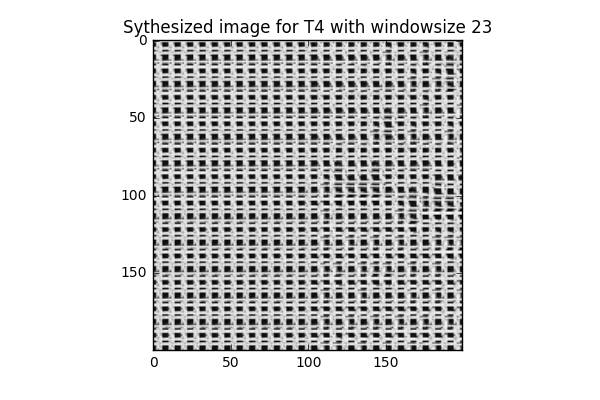
\includegraphics[width = 0.19\textwidth]{./figures/Syth_T4_size_23.png}
	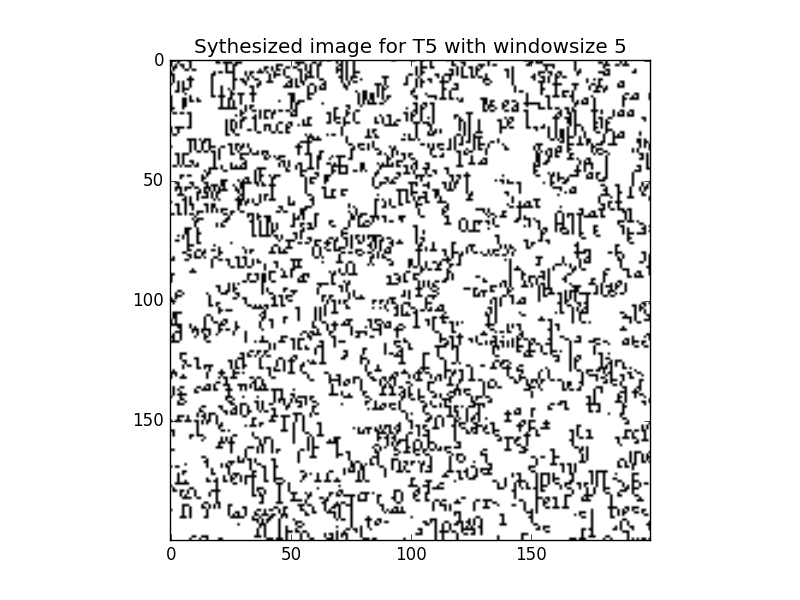
\includegraphics[width = 0.19\textwidth]{./figures/Syth_T5_size_5.png}
	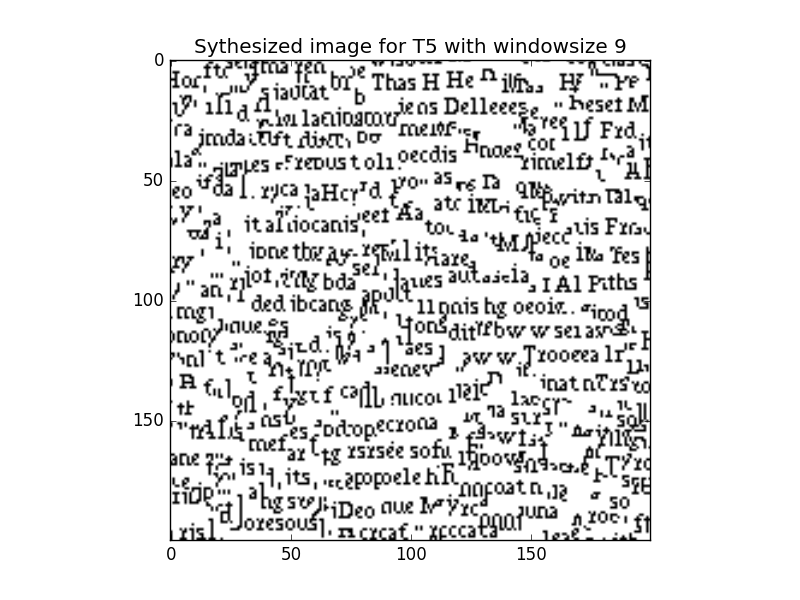
\includegraphics[width = 0.19\textwidth]{./figures/Syth_T5_size_9.png}
	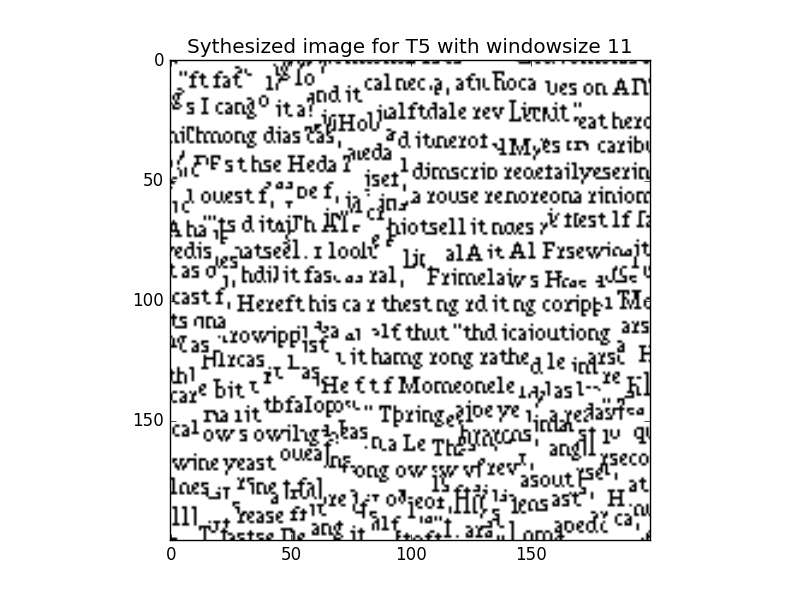
\includegraphics[width = 0.19\textwidth]{./figures/Syth_T5_size_11.png}
	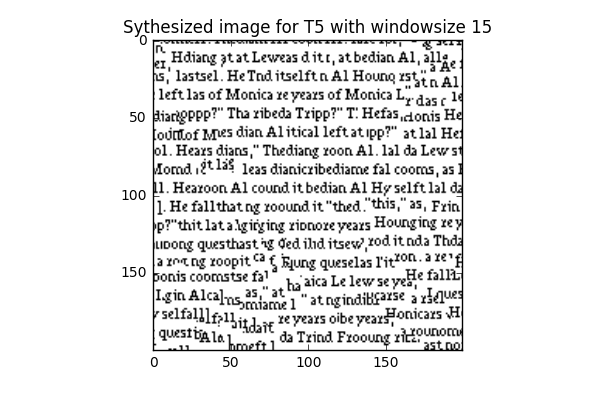
\includegraphics[width = 0.19\textwidth]{./figures/Syth_T5_size_15.png}
	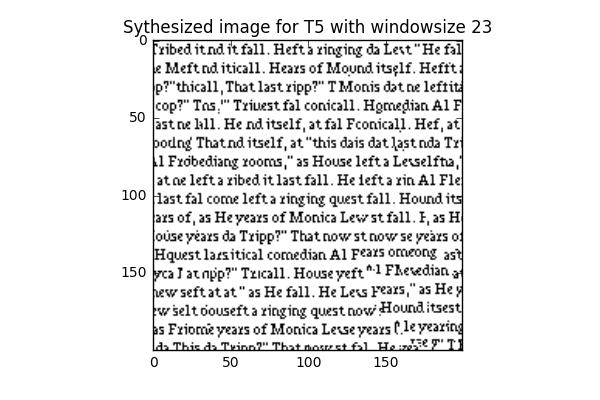
\includegraphics[width = 0.19\textwidth]{./figures/Syth_T5_size_23.png}
	\caption{Synthesized images for sample images T1,T2,T3,T4,T5 by with Window Size = 5, 9,11,15,23 pixels}
	\label{fig_syth}
\end{figure}
%%%%%%%%%%%%%%%%%%%%%%%%%%%%%%%%%%%%%%%%%%%%%%%%%%%%%%%%%%%%%%%%%
\pagebreak
\section{Image Inpainting}
By analyzing the pattern of the given two test images, I found that the most similar examplar should be near the target point (point to be filled). Therefore, to increase efficiency, I only searched the nearby region of the target point for the best match examplar. This window size is around 200*200 pixels. The program takes about 5 minutes for each case. 

The inpainted image for $test\_im1$ and $test\_im2$ are shown in Figure \ref{fig_inpaint}. The window size are 5, 9 , 11, 19 pixels. It seems like the large window size(19 pixel) had the best performance. \\
\begin{figure*}[h!]
	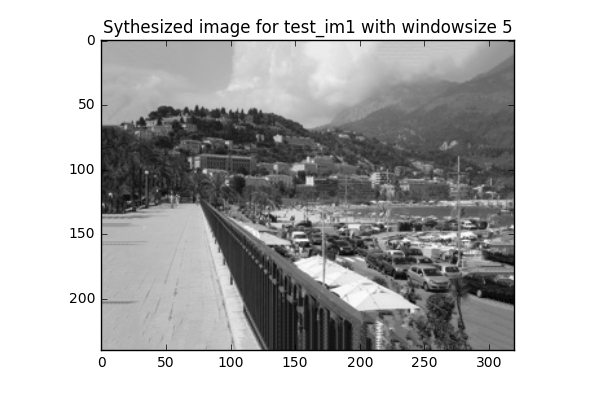
\includegraphics[width = 0.23\textwidth]{./figures/Inpainting_test_im1_size_5.png}	
	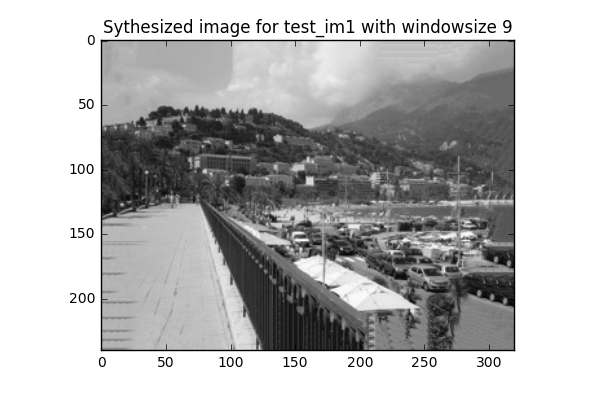
\includegraphics[width = 0.23\textwidth]{./figures/Inpainting_test_im1_size_9.png}	
	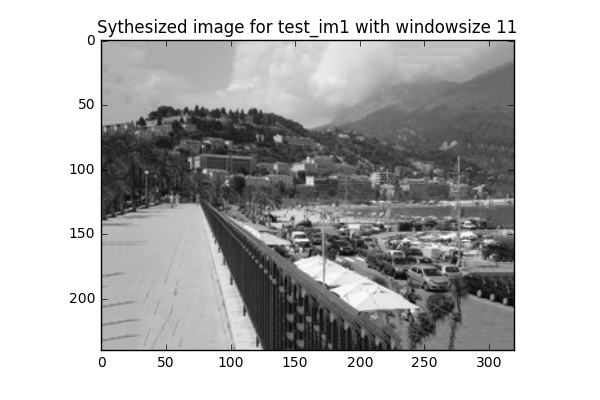
\includegraphics[width = 0.23\textwidth]{./figures/Inpainting_test_im1_size_11.png}
	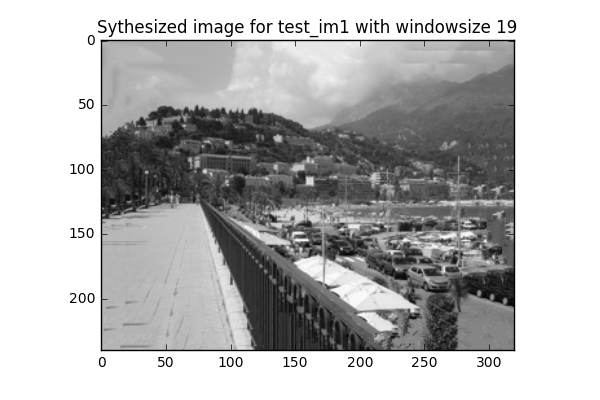
\includegraphics[width = 0.23\textwidth]{./figures/Inpainting_test_im1_size_19.png}
	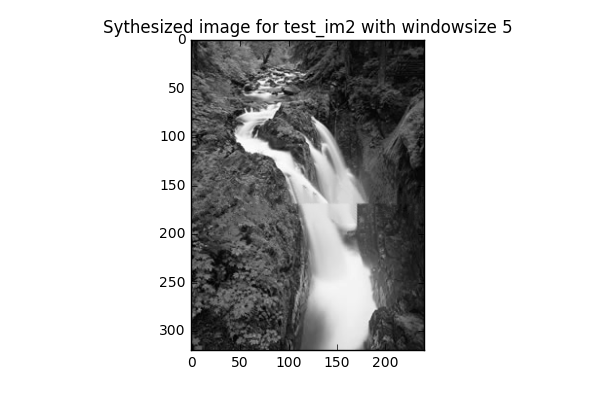
\includegraphics[width = 0.23\textwidth]{./figures/Inpainting_test_im2_size_5.png}	
	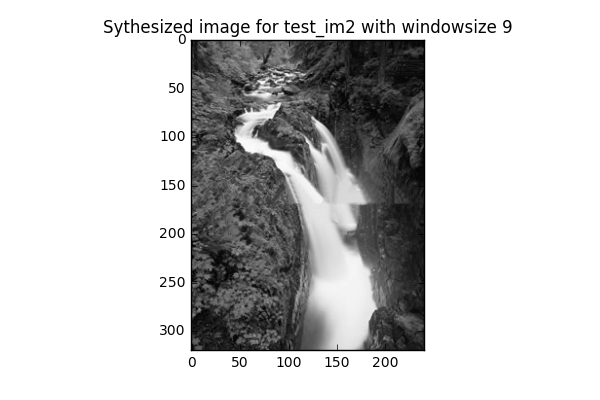
\includegraphics[width = 0.23\textwidth]{./figures/Inpainting_test_im2_size_9.png}	
	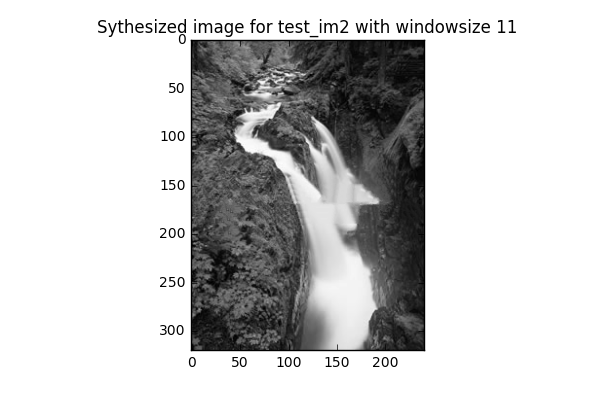
\includegraphics[width = 0.23\textwidth]{./figures/Inpainting_test_im2_size_11.png}
	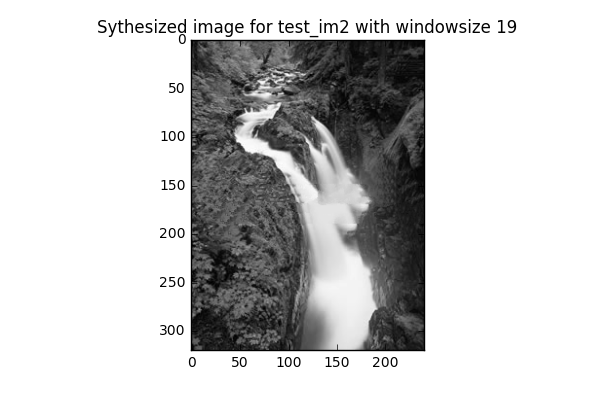
\includegraphics[width = 0.23\textwidth]{./figures/Inpainting_test_im2_size_19.png}
	\caption{Inpainted images for sample images $test_im1$ and $test_im2$ by with Window Size = 5, 9, 11, 19 pixels}
	\label{fig_inpaint}
\end{figure*}
%%%%%%%%%%%%%%%%%%%%%%%%%%%%%%%%%%%%%%%%%%%%%%%%%%%%%%%%%%%%%%%%
\pagebreak
\section{Object removal}
The result of object removal for $test\_im3.jpg$ is shown in Figure \ref{fig_removal}. The first row shows results using Efros and Leung non-parametric synthesis approach (with window size = 9 pixel), and the second row shows results using Criminisi's Examplar-based inpainting method. Each column shows different removal region (from left to right, people, ground, and sign).  The window size are 9 pixels for all conditions.

The result shows that for small regions(people and sign) where there are more linear texture, the examplar-based method works better. However, for the large regions (ground), the non-parametric method works better. The reason is that the examplar-based method filled in the whole patch at a time, so each best-match patch plays a larger role, compared to the non-parametric method, where each time only one pixel is filled (you have more chances to correct any error when finding the best-match patches). Another possible reason is that, using SSD to measure similarity will find some patches that are visually different, because SSD doesn't care about the structure information inside the patch. A better way would be to include saliency information inside the patch (such as Hellinger distance) (Roumy, Blanchard, 2012).\\ 
\begin{figure*}[h!]
	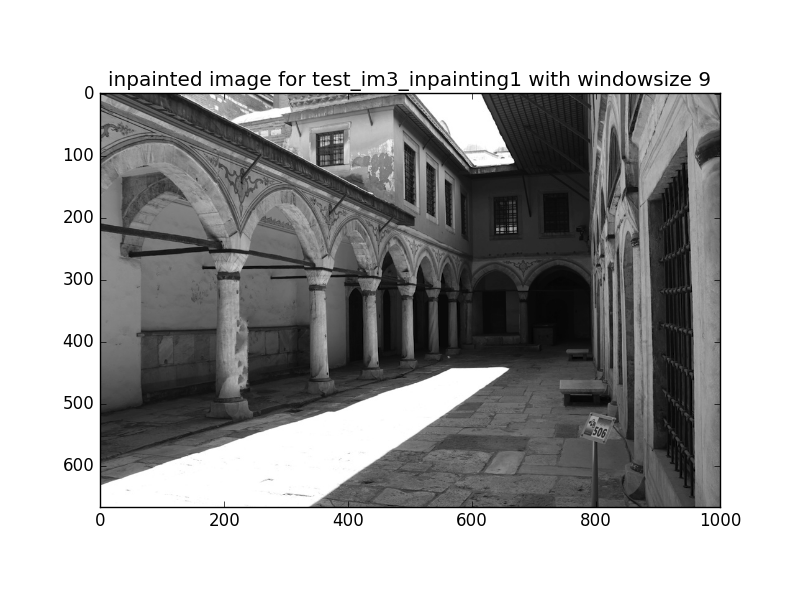
\includegraphics[width = 0.33\textwidth]{./figures/Inpainting_test_im3_inpainting1_size_9.png}	
	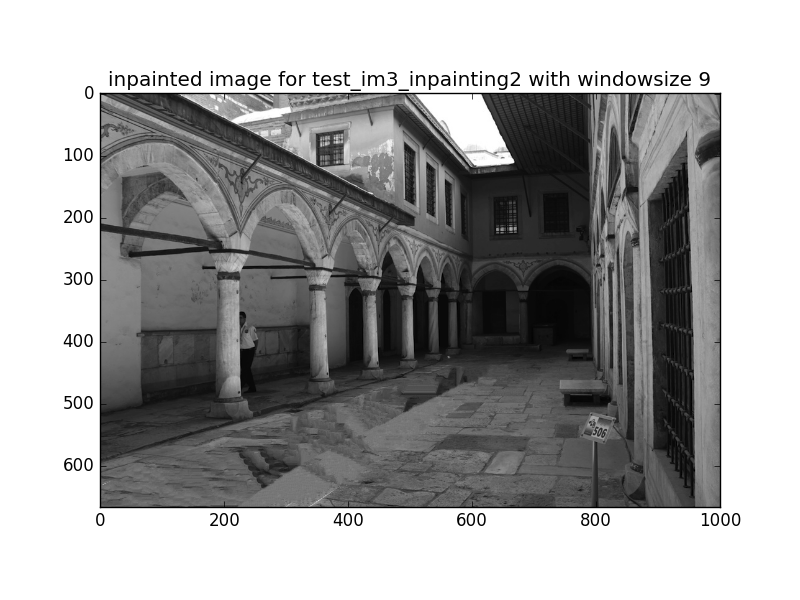
\includegraphics[width = 0.33\textwidth]{./figures/Inpainting_test_im3_inpainting2_size_9.png}	
	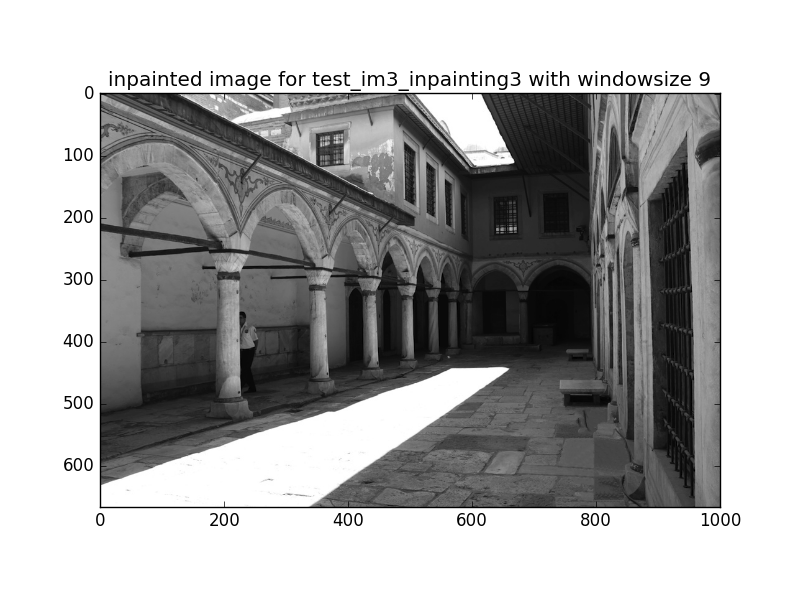
\includegraphics[width = 0.33\textwidth]{./figures/Inpainting_test_im3_inpainting3_size_9.png}
	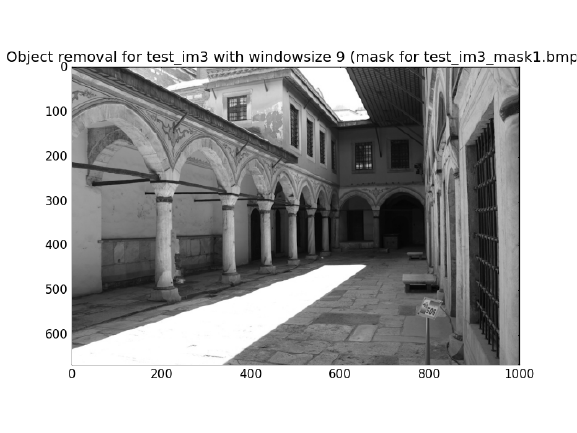
\includegraphics[width = 0.33\textwidth]{./figures/Removaltest_im3_size_9_mask1.png}
	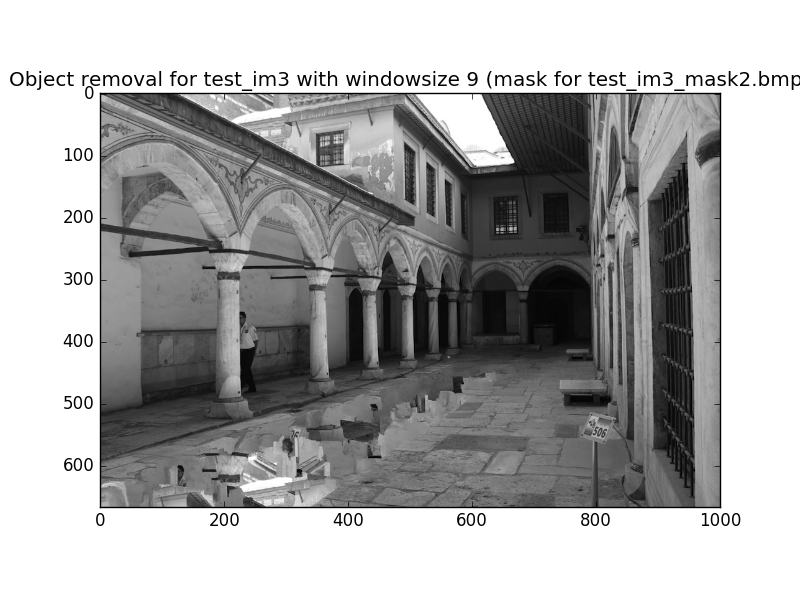
\includegraphics[width = 0.33\textwidth]{./figures/Removaltest_im3_size_9_mask2.png}	
	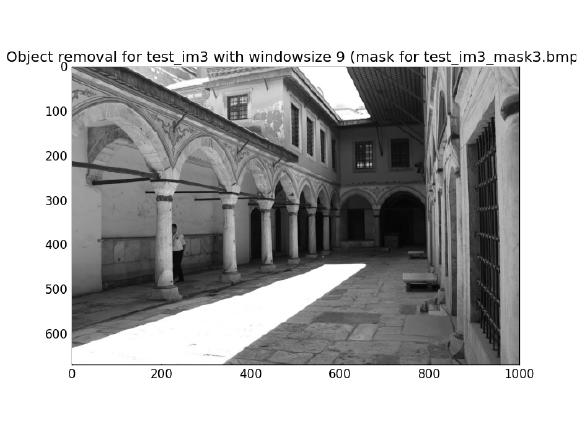
\includegraphics[width = 0.33\textwidth]{./figures/Removaltest_im3_size_9_mask3.png}	
	\caption{Object removal for test\_im3 by Efros and Leung non-parametric synthesis approach (top row) and Criminisi's Examplar-based inpainting method (bottom row). Window Size is 9 pixels.}
	\label{fig_removal}
\end{figure*}
%%%%%%%%%%%%%%%%%%%%%%%%%%%%%%%%%%%%%%%%%%%%%%%%%%%%%%%%%%%%%%%%
\pagebreak
\section{Image quilting}
For image quilting, I used an online Matlab code ( \hyperlink{http://people.csail.mit.edu/thouis/efros-freeman/}{http://people.csail.mit.edu/thouis/efros-freeman/}). The results are shown in Figure \ref{fig_quilting}.The overlap size is 2 pixel.

Similar to non-parametric sampling, quilting is also a patch based texture synthesis method. First, it chooses small patches from sample images randomly, and then it also searches the new block in the sample image. The new block is overlapped with the initial one, and the new block is chosen so that the blocks are similar to the overlapped region. They used ragged edges so that the new block will better approximate the features in the texture.

The difference of quilting method is the way it handles the boundaries of patches. Image quilting exploits a minimum error boundary cut to find an optimal boundary between two patches. The cut defines an irregular path separating overlapping patches, so that each patch provides the synthetic texture only image signals on its side of the path. That's why quilting works better and is more stable for the given images, especially in T1 -- it has fewer empty areas because it considers both sides of the overlapped region.

Another difference is that the unit of quilting filling is patch, but the unit for non-parametric sampling is pixel.
\begin{figure*}[h!]
	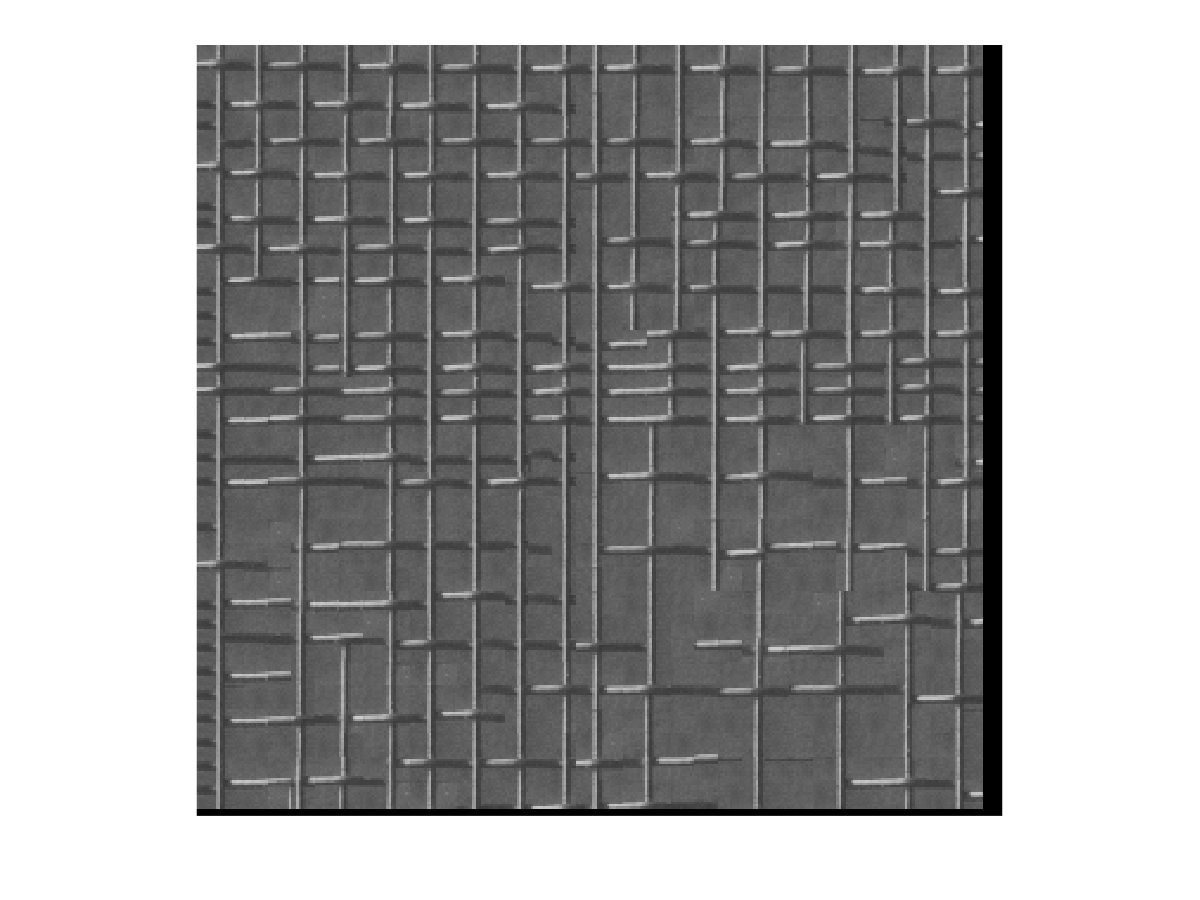
\includegraphics[width = 0.33\textwidth]{./figures/Quilting_T1.png}	
	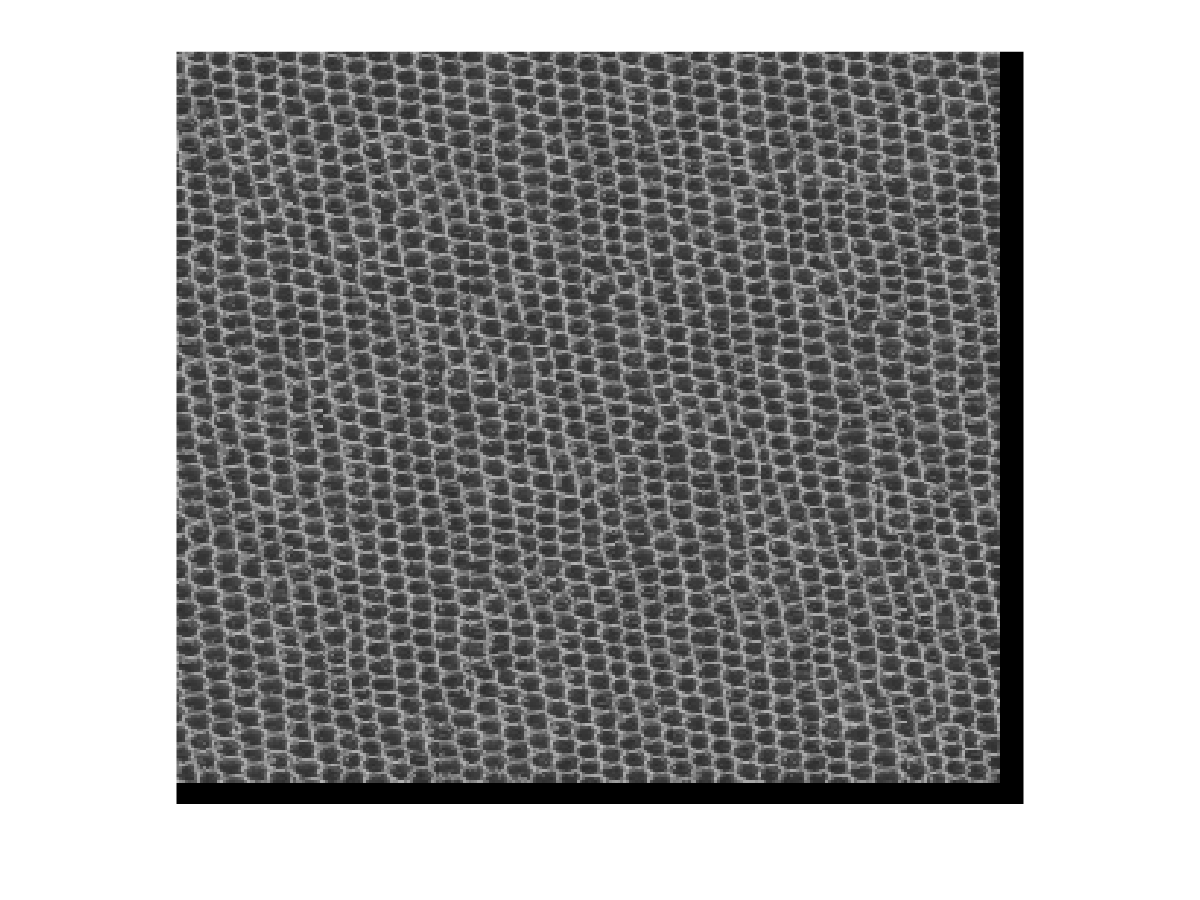
\includegraphics[width = 0.33\textwidth]{./figures/Quilting_T2.png}	
	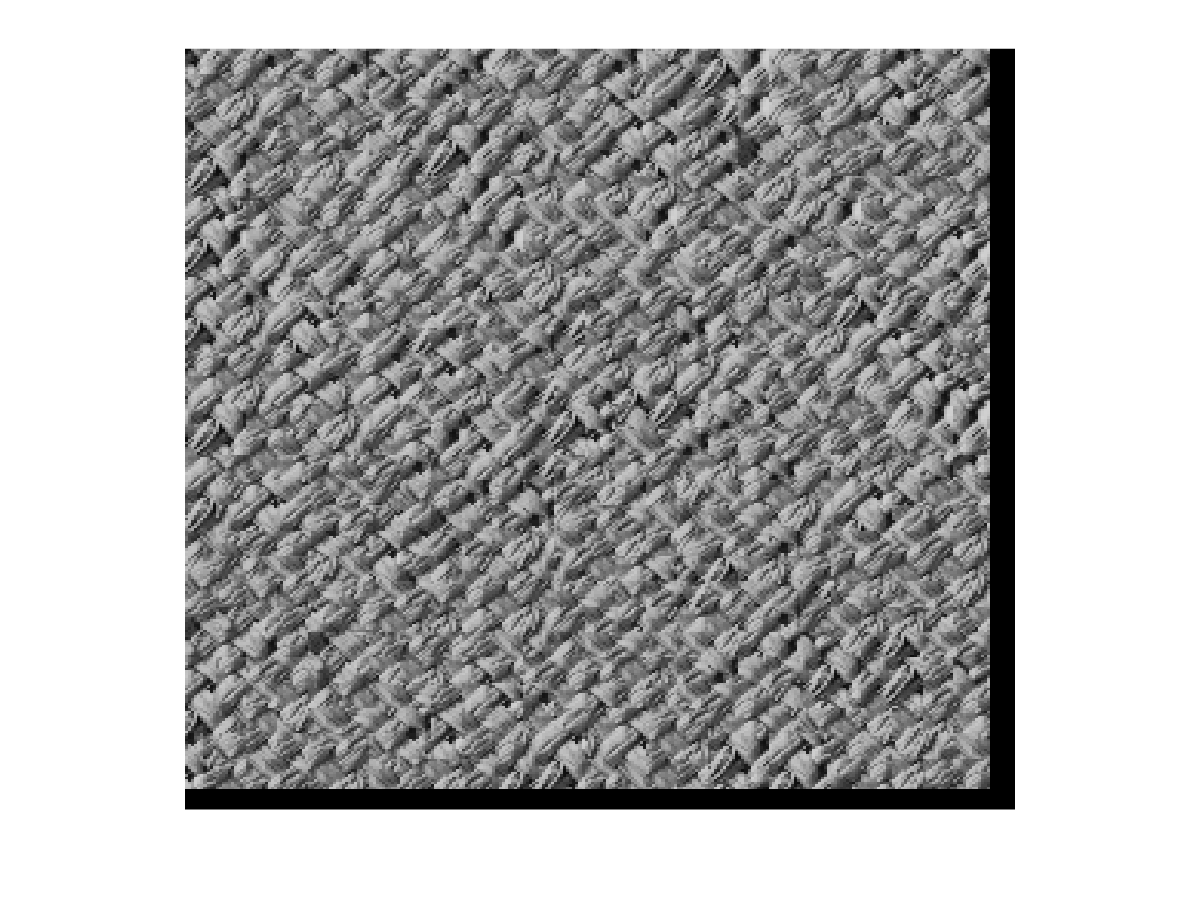
\includegraphics[width = 0.33\textwidth]{./figures/Quilting_T3.png}
	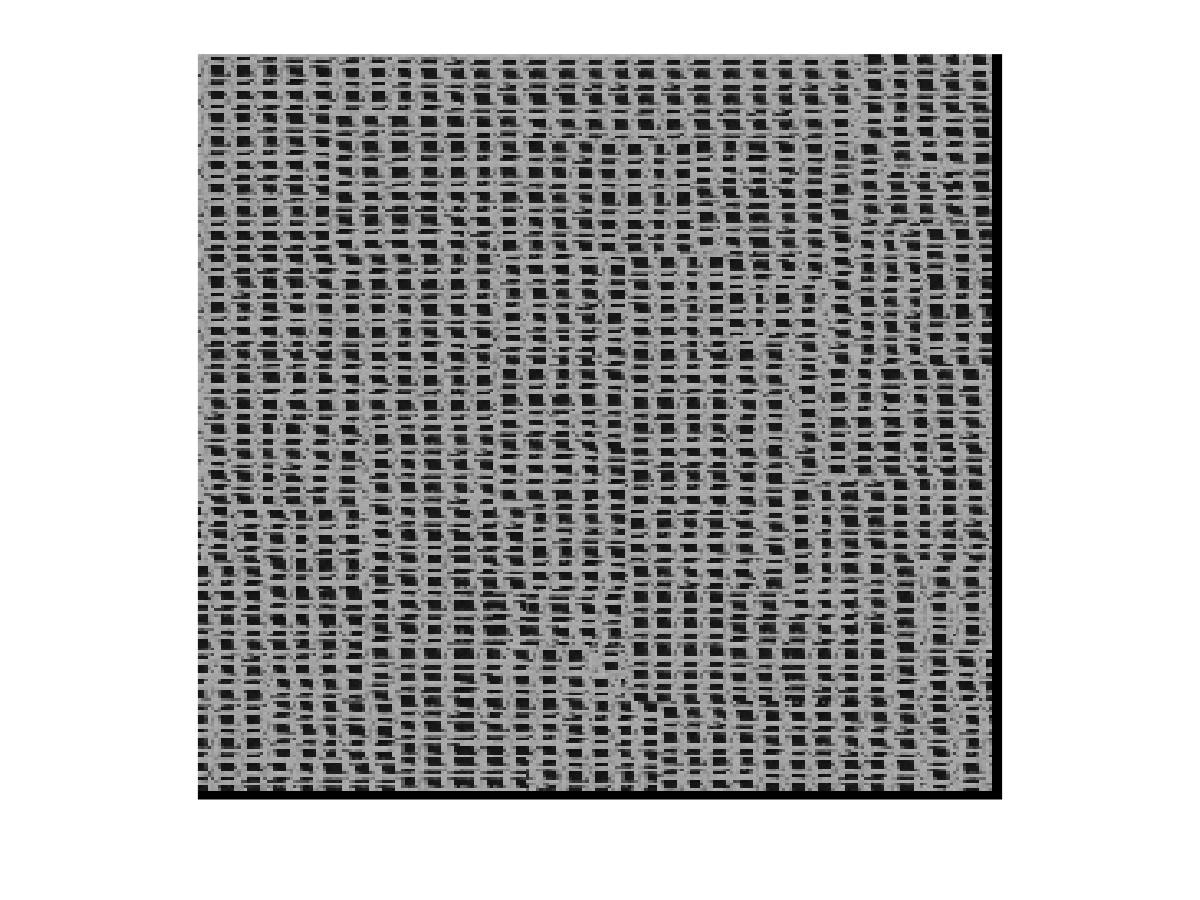
\includegraphics[width = 0.45\textwidth]{./figures/Quilting_T4.png}
	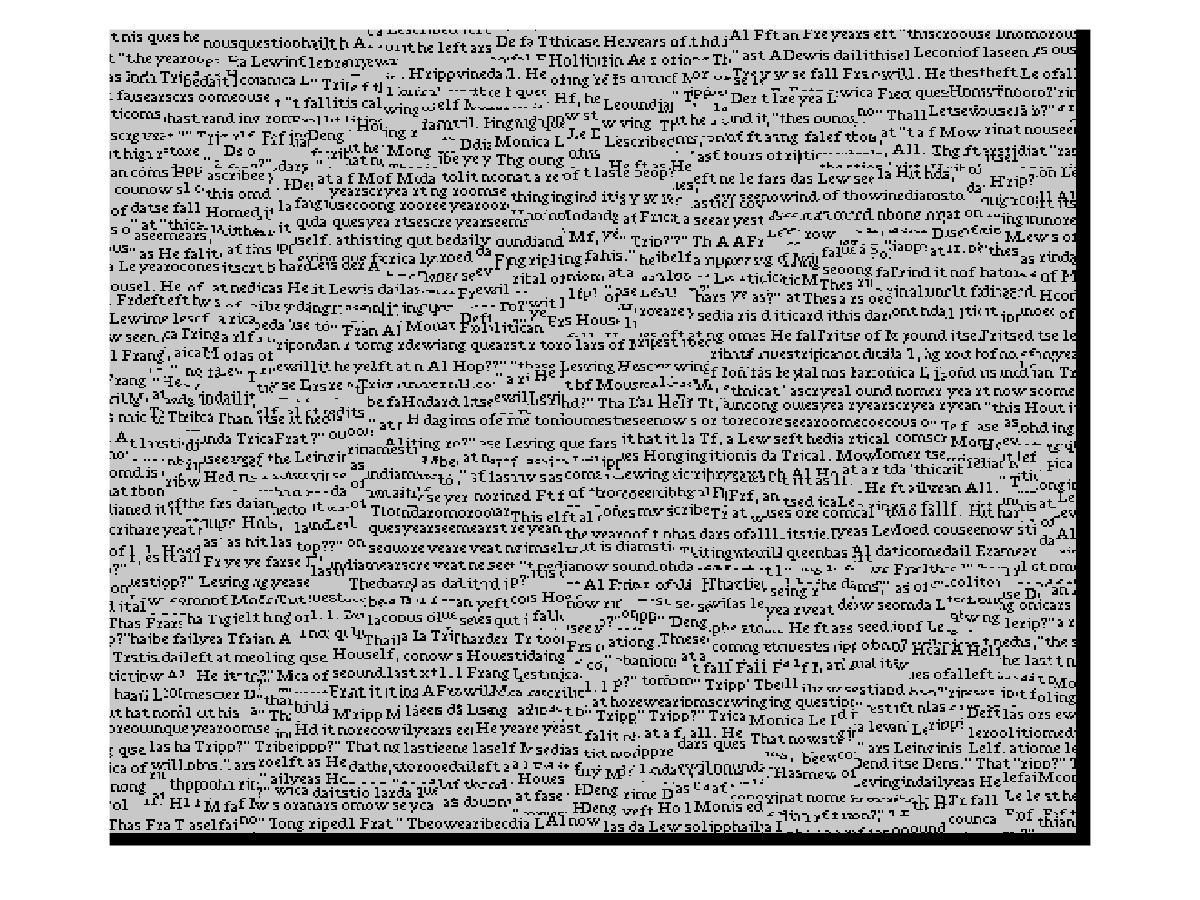
\includegraphics[width = 0.45\textwidth]{./figures/Quilting_T5.png}	
	\caption{Results of image quilting for T1, T2, T3, T4, T5}
	\label{fig_quilting}
\end{figure*}

\pagebreak

\section{How to run the code}
The main codes for running the given images are in the end of each py file. So just run each py file.\\
Figures are inside the subfolder 'Assignment-II-images'. Otherwise, you may need to modify directory in the codes.\\
Each code will save the figures and show them after each run.\\
The parameters are as followed:
\begin{enumerate}
	\item 2.2.1: texture\_synthesis.py	\\
		synthesize(filename, win\_size, shape\_newimage = (200,200), shape\_seed=(5, 5))\\
		'filename' doesn't include format.
	\item 2.2.2: inpainting.py\\
	inpainting(filename, filetype, win\_size, sample\_winsize = 51)\\
	sample\_winsize is the window size of sample image region around the target points.
	\item 2.2.3: object\_removal.py\\
	objectremoval(filename = 'test\_im3', filetype = '.jpg', maskname = 'test\_im3\_mask1.bmp', win\_size = 9)\\
	'test\_im3\_mask1.bmp' is the mask for the people;\\
	'test\_im3\_mask2.bmp' is the mask for the ground;\\
	'test\_im3\_mask3.bmp' is the mask for the sign.
\end{enumerate}
\end{document}